\section{A unified acceptance record and discriminating interventions}\label{sec:C33:07}
Across the three cases, an accepted artifact should be associated with a claim record containing the objective, applicable population, configuration, intervention, baseline, evidence, resource boundary, failure observations, and limits. This is not a generic success label. A passing patch, a grounded report, and an evolved harness require different validators, but each needs a trace from the delivered artifact to the evidence that supports it.

\begin{table}[!htbp]
\centering
\caption{Cross-layer failure hypotheses and discriminating interventions.}\label{tab:C33:interventions}
\begin{tabular}{L{0.24\linewidth}L{0.30\linewidth}L{0.32\linewidth}}

\toprule Coupling failure & Targeted intervention & Discriminating observation\\\midrule
Context omits a constraint & Preserve or remove only the qualifier & Action changes while unrelated content is fixed.\\
Memory is stale & Swap valid and superseded records & Temporal resolution and authority behavior differ appropriately.\\
Cache reuse is invalid & Alter one prefix dependency & Fresh and reused computations diverge beyond declared tolerance.\\
Harness search overfits & Freeze candidate and change population & Selection gains fail to transfer under matched resources.\\
Verifier misses a requirement & Add a requirement-derived hidden check & Previously accepted artifacts reveal a specific false acceptance.\\
Rollback restores revoked state & Revoke after checkpoint, then recover & Recovery preserves current authority and deletion constraints.\\
\bottomrule
\end{tabular}
\end{table}

The interventions are narrow enough to falsify mechanism explanations. They also expose where an observed improvement is underdetermined. If a structured-memory system changes storage, retrieval, prompting, and maintenance simultaneously, an end-to-end gain does not identify which component caused it. Factorial ablations or staged replacements can locate the contribution, while a complete system comparison remains useful for deployment decisions. Mechanistic attribution and engineering utility are different questions.

Cross-layer work should report the simplest baseline that survives these tests. An event log plus deterministic metadata can outperform an elaborate reflective memory on tasks dominated by exact state. A reactive policy with a strong tool interface can outperform search when observations are reliable and actions cheap. A single agent can outperform a team when coordination consumes the available context and latency budget. These are conditional possibilities to test, not universal rankings. The value of the system formulation is that it makes those conditions visible and turns a broad claim about autonomy into a set of specific, reviewable technical propositions.


Figure~\ref{fig:C33:overview} isolates the mechanism and its stated information boundaries.
\begin{figure}[!htbp]
\centering
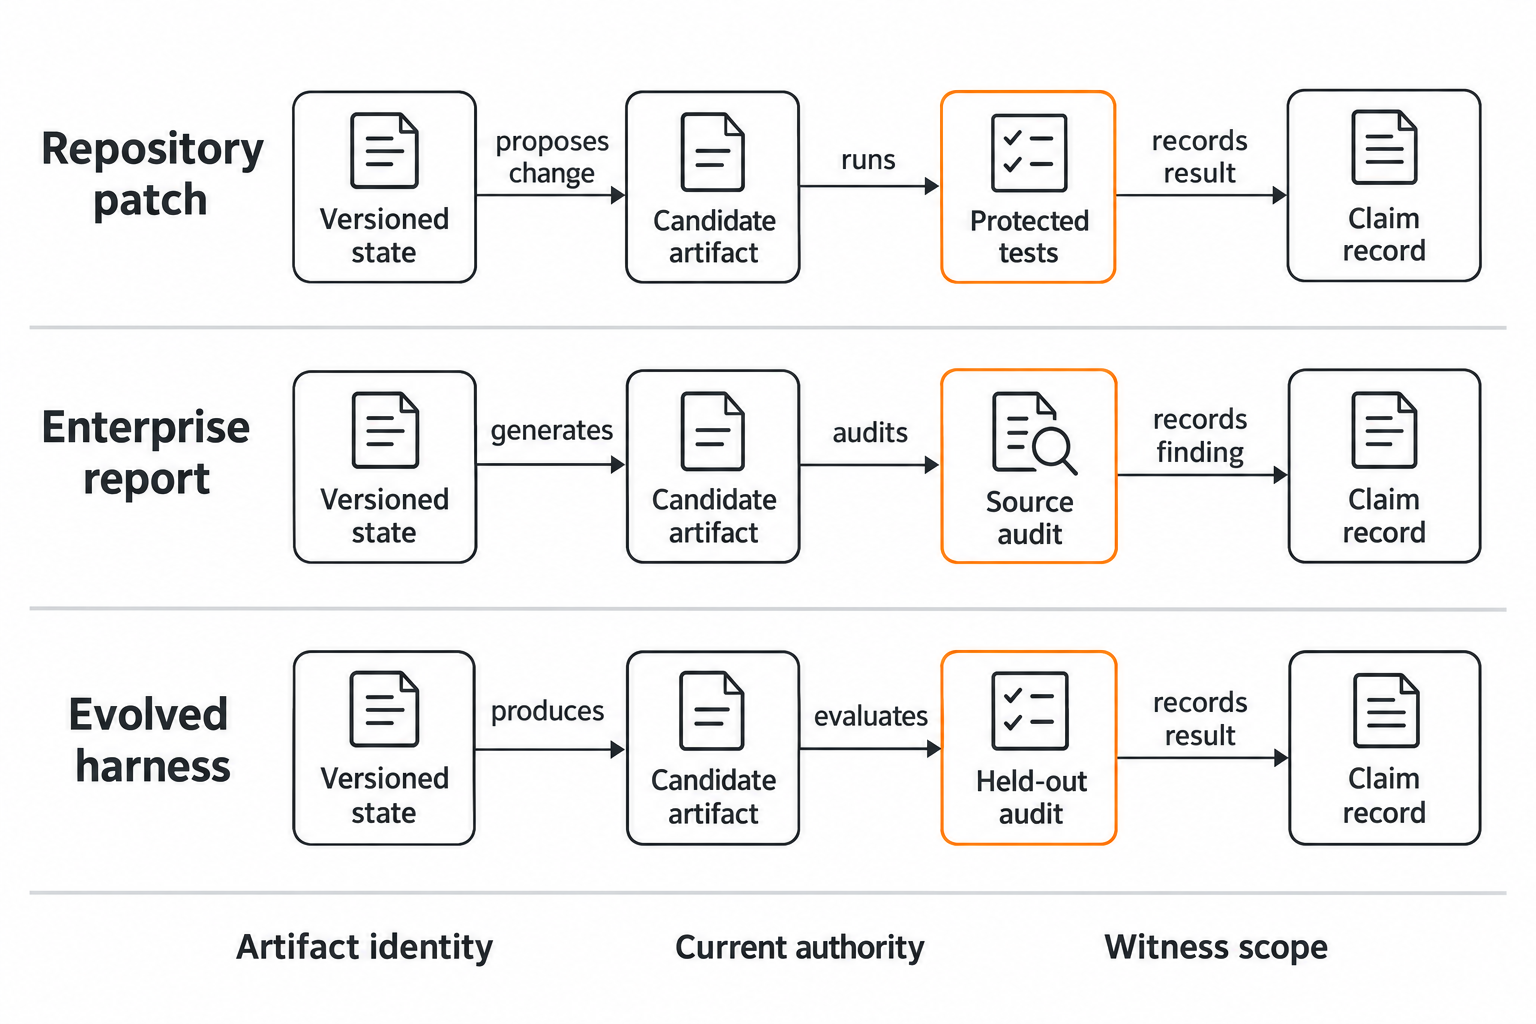
\includegraphics[width=\linewidth]{book/figures/assets/F33review.png}
\caption{The constructed workflows require different witnesses: protected behavior checks, source-level review, or held-out evaluation. Each claim record binds the delivered artifact to its versioned state, current authority and actual witness scope. A passing local check does not certify the complete workflow.}
\label{fig:C33:overview}
\end{figure}
